% 
% 
% 
% 
% 
% \documentclass[runningheads,a4paper]{llncs}
% \usepackage[T1]{fontenc}
% \usepackage{amssymb}
% \usepackage{cite}
% \setcounter{tocdepth}{3}
% \usepackage{graphicx}
% \usepackage{subfig}
% \usepackage[capitalize,noabbrev,nameinlink]{cleveref}
% 
% \usepackage{url}
% \usepackage{amsmath} 
% \usepackage{mathtools} 
% %\usepackage{qtree}
% \usepackage{multirow}
% \usepackage{relsize}
% \usepackage{authblk}
% \usepackage{placeins}
% 
% 
% 
% \usepackage{tikz}
% \usetikzlibrary{shapes}
% 
% \usepackage{xspace}
% \newcommand{\A}{\ensuremath{\mathcal{A}}\xspace}
% \newcommand{\B}{\ensuremath{\mathcal{B}}\xspace}
% \newcommand\pa[1]{\ensuremath{\left(#1\right)}}
% 
% 
% 
% 
% 
% 
% 
% 
% 
% 
% 
% 
% 
% % Graphics
% \usepackage{graphicx}
% \setcounter{bottomnumber}{2}
% \usepackage{tikz}
% \usetikzlibrary{arrows,positioning,shapes.misc,calc}
% \definecolor{lightgrey}{RGB}{170, 170, 170}
% \pgfdeclarelayer{background}
% \pgfdeclarelayer{foreground}
% \pgfsetlayers{background,main,foreground}
% \usepackage{pgf-umlsd}
% 
% 
% 
% 
% 
% % Listings and Verbatim environment
% \usepackage{fancyvrb}
% \usepackage{relsize}
% \usepackage{listings}
% \usepackage{verbatim}
% \usepackage{alltt}
% \newcommand\listingsize{\fontsize{9pt}{10pt}}
% \RecustomVerbatimCommand{\Verb}{Verb}{fontsize=\listingsize}
% \RecustomVerbatimEnvironment{Verbatim}{Verbatim}{fontsize=\listingsize}
% \lstset{frame=lines,captionpos=b,numberbychapter=false,escapechar=§,
%         % line numbers
%         numbers=left,
%         numbersep=2ex,
%         numberstyle=\textcolor{lightgrey},
%         xleftmargin=5ex,
%         framexleftmargin=5ex,
%         aboveskip=0.5em,
%         % font style
%         basicstyle=\ttfamily\listingsize\selectfont}
% %\crefname{lstlisting}{Listing}{Listings}
% \definecolor{grey}{RGB}{130,130,130}
% 
% 
% 
% 
% 
% 
% 
% 
% 
% 
% 
% 
% 
% 
% % Acronyms
% \usepackage{xspace}
% \newcommand{\apis}{\mbox{{API}s}\xspace}
% \newcommand{\api}{{API}\xspace}
% \newcommand{\dbpedia}{DBpedia\xspace}
% \newcommand{\cwm}{{\itshape cwm}\xspace}
% \newcommand{\http}{{HTTP}\xspace}
% \newcommand{\notationthree}{Notation3\xspace}
% \newcommand{\nthree}{{N\oldstylenums 3}\xspace}
% \newcommand{\nthreelogic}{N{\oldstylenums 3}Logic\xspace}
% \newcommand{\owls}{\mbox{OWL-S}\xspace}
% \newcommand{\rdf}{RDF\xspace}
% \newcommand{\rest}{REST\xspace}
% \newcommand{\restdesc}{RESTdesc\xspace}
% \newcommand{\sla}{SLA\xspace}
% \newcommand{\soap}{SOAP\xspace}
% \newcommand{\uri}{URI\xspace}
% \newcommand{\uris}{URIs\xspace}
% \newcommand{\iri}{IRI\xspace}
% \newcommand{\URL}{URL\xspace}
% \newcommand{\wsmo}{WSMO\xspace}
% \newcommand{\wwwc}{W3C\xspace}
% 
% 
% 
% 
% 
% 
% 
% 
% 
% 
% 
% 
% 
% 
% 
% 
% 
% %\setlength{\textfloatsep}{10pt plus 100.0pt minus 10.0pt}
% 
% 
% \begin{document}
% 
% \mainmatter
% 
% \title{ Improving OWL RL reasoning in N3 by using specialized rules}
% \author{D\"orthe Arndt\inst{1}%
% %\thanks{}%
% \and Ben De Meester \inst{1} \and Pieter Bonte\inst{2} \and Jeroen Schaballie\inst{2}\and
% Jabran~Bhatti\inst{3} \and  Wim Dereuddre\inst{3} 
% \and Ruben Verborgh\inst{1} \and Femke Ongenae\inst{2} \and Filip~De~Turck\inst{2} \and  Rik Van de Walle\inst{1} \and Erik Mannens\inst{1}}
% %
% \authorrunning{D\"orthe Arndt et al.}
% 
% % the affiliations are given next; don't give your e-mail address
% % unless you accept that it will be published
% \institute{Ghent University -- iMinds -- Multimedia Lab, Belgium\\
% \email{\{doerthe.arndt, ben.demeester, ruben.verborgh\}@ugent.be}
% \and
% IBCN research group, INTEC, Ghent University -- iMinds, Belgium\\
% \email{\{pieter.bonte, jeroen.schaballie, femke.ongenae\}@intec.ugent.be}
% \and
% Televic Healthcare, Belgium\\
% \email{\{j.bhatti, w.dereuddre\}@televic.com}
% }
% 
% 
% \maketitle
% 
% 
% \begin{abstract}
% Semantic Web reasoning can be a complex task: depending on the amount of data and the ontologies involved, traditional OWL DL reasoners can be too slow
% to face %real life 
% problems in real time. An alternative is to use a rule-based reasoner together with the OWL RL/RDF rules as stated in the specification of the OWL 2 language profiles.
% In most cases this approach actually improves reasoning times, but due to the complexity of the rules, not as much as it could. 
% In this paper we present an improved strategy: based on the TBoxes of the ontologies involved in a reasoning task, we create more specific rules which 
% then can be used for further reasoning. We make use of the EYE reasoner and its logic Notation3. In this logic, 
% rules can be employed to derive new rules which makes 
% the rule creation a reasoning step on its own. We evaluate our implementation on a semantic nurse call system.
% Our results show that adding a pre-reasoning step to produce specialized rules improves reasoning times by around 75\%.
% 
% 
% \keywords{Notation3, rule-based reasoning, OWL 2 RL} 
% \end{abstract}


\subsection{Introduction}
With the increasing amount of
 carefully designed ontologies
semantic web reasoning is becoming more popular for industrial applications:  
ontologies can be employed to solve complex problems in domains like medicine, automotive industry 
or finance (e.g., \cite{finance}, \cite{snomed2}). 
Nevertheless, there are still some obstacles which hinder semantic web reasoning from being fully established. One of these is scalability: 
depending on the amount of data and the ontologies involved, traditional OWL DL reasoners can be too slow
to solve 
problems in real time. The different OWL 2 profiles \cite{OWLRL} provide a solution: by
using less expressive but still powerful subsets of OWL DL, reasoning times can be significantly improved.

In this paper we focus on the OWL RL profile which 
is designed to enable rule-based reasoners
to draw the right conclusions from ontology data and concepts. 
The rules for that, as presented in the specification, are complex 
in the sense that they rely on rather complicated patterns occurring in both ABox and TBox which have to be found to draw conclusions.
We propose to improve 
OWL RL reasoning performance 
by adding an extra reasoning 
step. Based on the ontology's TBox, specialized rules can be automatically 
produced to be used for further reasoning on the ABox. 
Due to its expressiveness we use Notation3 Logic \cite{N3Logic} to perform this task.
The highly performant
EYE reasoner \cite{eyepaper} 
is used for reasoning.
As our pre-reasoning step has to be executed only once for every TBox, our approach is especially suitable for situations where the 
same reasoning has to be performed on frequently changing data. We %therefore 
tested our implementation in an event based reasoning set-up: a semantic
nurse call system which controls the technical equipment in a hospital and, for example, assigns the most suitable nurse to a patient's call.
Our tests showed that our pre-reasoning step reduces reasoning times at about 75\% compared to an implementation using the originally proposed rules.



The remainder of this paper is structured as follows: in \cref{relwork} we give an overview of related work. After that, in \cref{usecase}, we explain 
our use case, a semantic nurse call system. \cref{owlrl} gives a general introduction to OWL RL in N3. In \cref{reasoning} we describe our system in more detail, 
focusing in particular on the improved rules themselves and 
 the steps which are necessary to produce them. An evaluation of our implementation is given in \cref{ev}. We summarize our main findings and 
give an outlook to future work in \cref{conc}.


% \subsection{Related Work}\label{relwork}
% 
% 
% Traditionally, reasoning over OWL ontologies was performed by description logic based reasoners using (variants of) the tableaux algorithm.
% Prominent examples of such reasoners are Pellet \cite{Pellet} and HermiT \cite{hermit}. 
% Both support---as others of their kind---the full OWL DL profile. The expressiveness of this profile and the complexity of the related reasoning,
% make these reasoners perform rather slow in comparison with, for example, rule-based reasoners. The OWL 2 profiles \cite{OWLRL} aim to overcome this gap 
% by defining less expressive
% but still powerful subsets of OWL DL. One of these profiles is OWL RL, which was designed to enable rule-based reasoners to cope with OWL ontologies. 
% Various implementations make use of 
% the OWL 2 RL/\rdf rules as proposed in the specification, among them
%  OWLim \cite{owlim} and Oracle's RDF Semantic Graph \cite{oracle}. 
% As most other implementations we are aware of, these reasoners support their own rule format, 
% and optimizations are done internally using
% the underlying programming language. 
% We propose an optimization which can be done in the logic itself by performing an extra reasoning step.
% We are thereby independent of a specific reasoner.
% 
%  
%  
% Notation3 Logic (\nthree) was introduced in 2008 by Tim Berners-Lee et al. \cite{N3Logic}.
% It forms a superset of \rdf and extends the \rdf data model by formulas (graphs), functional predicates, universal variables and logical operators, in particular
% the implication operator. Rules in \nthree can not only be applied to derive new \rdf triples, it is also possible to write and apply rules with new rules in 
% their consequence, and thus to derive new rules. It is exactly this property which made us opt for using \nthree instead of other 
% rule formats like, e.g., SWRL \cite{swrl}.
% 
% There are several reasoners supporting \nthree:
% FuXi \cite{fuxi} is a forward-chaining production system for Notation3 whose reasoning is based on the RETE algorithm. 
% The forward-chaining cwm \cite{cwm} reasoner 
% is a general-purpose data processing tool which can be used for querying, checking, transforming 
% and filtering information.
% EYE \cite{eyepaper} is a reasoner which is enhanced with Euler path detection. 
% It supports 
% backward and 
% forward 
% reasoning and also a user-defined mixture of both. 
% Amongst its 
% numerous features are the option to skolemize blank nodes
% and  the possibility to produce and reuse proofs for further reasoning. 
% The reason why we use EYE in our implementation is its high performance. 
% Existing benchmarks and results are listed in the above-mentioned paper \cite{eyepaper} and on the EYE website \cite{eye}.
% 


 

% \subsection{Use Case}\label{usecase}
% Our use case is a nurse call system in a hospital.
% The system is aware of certain details about personnel and patients represented in an OWL ontology.
% Such information can include: personal skills of a staff member, staff competences, patient information, special patient needs, and/or the 
% personal relationship between staff members and patients. 
% Furthermore, there is dynamic information available, for example, the current location of staff members and their status (busy or free). 
% When a call is made, the nurse
% call system should be able to assign the best staff member to answer that call. The definition of this ``best'' person
% varies between hospitals and can be quite complex. 
% The system additionally controls different devices. If for example staff members enter a room with a patient, 
% a light should be switched on; if they log into the room's terminal, they should have access to the medical lockers in the room. 
% The event-driven reasoning system for this use case has to fulfill certain requirements.
% \begin{description}
% \item[scalability] It should cope with data sets ranging from 1000 to 100,000 relevant triples (i.e., triples necessary to be included for the reasoning to be correct). 
% Especially in bigger hospitals the number of staff members and patients and thereby also the amount of available information about those can be quite big. 
% It is not always possible to divide this knowledge into smaller independent chunks as this data is normally full of mutual dependencies. 
% \item[functional complexity] It should implement deterministic decision trees with varying complexities. The reasons to assign a nurse to 
% a certain patient can be as manifold as the data. Previous work has shown that this complexity is not only theoretically possible but also desired by the 
% parties interested in such a semantic system~\cite{accioont}.
% \item[configuration] It should support the ability to change these decision trees at configuration time. Different hospitals have different 
% requirements and even in one single hospital those requirements 
% can easily change due to e.g., an increase of available information or a simple change in the hospital's organizational concepts or philosophy.
% \item[real-time] It should return a response within 5 seconds to any given event. Especially in such a delicate sector as patient care, seconds can make a difference. 
% Even though a semantic nurse call system will not typically be employed to assign urgent emergency calls  through complex decision trees, 
% a patient should not wait too long till his possibly pressing request is answered.
% \end{description}
% The functional complexity requirement together with the configuration constraint motivate 
% the choice of a reasoning system which supports rules as these can be seen as the most natural way to 
% express decision trees. Even though a numerous amount of OWL DL reasoners support at least one rule format, 
% their reasoning is too slow to meet the scalability and the real-time constraint \cite{ORCA}. \todo{that is the paper used for the first part of this section, so remove reference!}
% Therefore, we chose a rule-based solution. 
%  

\subsection{OWL RL in N3}\label{owlrl}
\hyphenation{EYE ACCIO}

 

In a first attempt to solve the above-mentioned problem we used a direct translation of OWL 2 RL/\rdf rules as listed on the corresponding website~\cite{OWLRL}. 
Where possible, we made use of existing N3-translations of these rules as provided by EYE~\cite{EYEowl}. Missing concepts were added. 
The data was represented using the ACCIO ontology \cite{accioont} which will be further described in section \ref{ont}.
The results of this 
implementation were already promising \cite{arndt_ruleml_2015},\todo{replace reference} but for larger data sets the reasoning took multiple minutes and, thus, did not meet the requirements claimed above. 

We explain the idea behind these OWL RL rules in \nthree and how they can be improved using
%We start with 
an example: Listing~\ref{lst:subclass} shows 
the class axiom rule\footnote{The rule is the N3 version of the cax-sco rule in Table 7 on the OWL 2 Profiles website~\cite{OWLRL}.} which is needed 
to deal with the rdfs concept  \verb!subclassOf!.
For convenience we omit the prefixes in the formulas below. The empty prefix refers to the ACCIO ontology, 
 \verb!rdf! and \verb!rdfs! have the same meaning as in Listing~\ref{lst:subclass}. Consider that we have the following TBox triple stating that the class \verb!:Call!
 is 
 a subclass of the class \verb!:Task!:
\[
 \verb!:Call rdfs:subClassOf :Task.! \tag{1}\label{1}
\]
If the ABox contains an individual which is member of the class \verb!:Call!
\[\verb! :call1 a :Call.! \tag{2}\label{2}\]
an OWL DL reasoner would make the conclusion that the individual also belongs to the class \verb!Task!: 
\[
 \verb!:call1 a :Task.! \tag{3}\label{3}
\]
Our rule in Listing \ref{lst:subclass} does exactly the same: as Formula~\ref{1} and Formula~\ref{2} can be unified with the antecedent of the rule, a reasoner derives
the triple in Formula~\ref{3}. 
%
But this unification is rather expensive: if we take a closer look to the antecedent we see that it contains three different variables occurring 
in two different triples which have to be instantiated with the data of the ontology. In our use case information as stated in 
Formula~\ref{2} can change---patients will make new calls---but statements as Formula~\ref{1} can be considered as fixed: the terminology does not change during the reasoning process,
calls are tasks for our ontology. Our solution makes use of this observation: what is valid for the triple in Formula~\ref{1} also counts for other TBox-triples. We consider the
TBox as static knowledge which can be used for pre-processing. The idea of our solution is to do as much unification as possible before dealing with (possibly) dynamic data. 
We produce more specialized rules, in the case mentioned above, for example the rule
%
\[
\verb!{?X a :Call.} => {?X a :Task.}.!
\tag{4}\label{4}
\]
which will derive for every new call, that it is also a task, just as the rule in Listing~\ref{lst:subclass} does.











\subsection{Producing TBox-rules}\label{reasoning}
In order to achieve the goal explained in the last section, producing specialized rules based on the concepts present in the ontology's TBox, 
we use the EYE reasoner.
Reasoning in EYE can be considered as a single  process, having as input all necessary files representing the knowledge 
(i.e., the necessary ontologies, data, and rule-files), and a query-file that filters the output of the reasoning result.
We have to perform two steps:
\begin{enumerate}
 \item Produce a grounded copy of the  TBox. 
 \item Use rules to translate the grounded TBox into specialized rules.
\end{enumerate}

The need of the first step has to do with the fact that an ontology can contain anonymous classes represented by blank nodes. Used in rules, 
these blank node class names have, due to the semantics of \nthree, a 
limited scope. It is therefore difficult to use them to reference the same class in different rules. 
We will give a more elaborate explanation in the next section. 
After that we will describe the translation step in more detail.



\subsubsection{Grounding the Ontology}
\begin{lstlisting}[
  float=t,
  caption={ACCIO example: a call is both, a patient task and an unplanned task. },
  label=task]
§\textcolor{gray}{@prefix : <http://ontology/Accio.owl\#>.}§
§\textcolor{gray}{@prefix owl: <http://www.w3.org/2002/07/owl\#>.}§
§\textcolor{gray}{@prefix rdf: <http://www.w3.org/1999/02/22-rdf-syntax-ns\#>.}§
§\textcolor{gray}{@prefix rdfs: <http://www.w3.org/2000/01/rdf-schema\#>.}§

:Call  rdfs:subClassOf [ 
                       rdf:type owl:Class ;
                       owl:intersectionOf ( 
                                     :PatientTask
                                     :UnplannedTask
                                   )
                       ].
\end{lstlisting}


Before translating the TBox into rules we have to replace all blank nodes by \uris or literals. To understand the reason for this skolemization step, 
consider the example in Listing~\ref{task}.
The example contains triples which further describe the class \texttt{:Call} from Formula~\ref{2}.
A call is a patient task and an unplanned task, or to be more specific:
the class \texttt{:Call} is subclass of an anonymous class which is the intersection of 
the classes \texttt{:PatientTask} and \texttt{:UnplannedTask}. 
Even though \nthree supports rules which contain blank nodes, it is exactly this anonymous class which causes problems. 
Being unlabeled, the blank node can be referred by an arbitrary new blank node name. A translation as done in Formula~\ref{4} would result in a rule like:
\[
\verb!{ ?X a :Call. } => { ?X a _:newblank.}.! 
\tag{5}\label{newblank}
\]
This rule means, that every instance of the class \texttt{:Call} is also instance of \textit{some} other class. 
This knowledge can already be gained by Formula~\ref{4} and does 
not have much influence 
on further reasoning. And even if the blank node in Listing~\ref{task} would be labeled by, for example, \texttt{\_:intersection1} a new rule
\[
\verb!{ ?X a :Call. } => { ?X a _:intersection1.}.! 
\tag{6}\label{union}
\]
would have no other meaning than Formula~\ref{4} as in \nthree the scope of a blank node is always only the graph, i.e. the curly brackets \texttt{\{ \}}, 
in which it occurs  \cite{Notation3, arndt_ruleml_2015}. 
The consequence of the rule would not refer to our intersection of patient tasks and unplanned tasks.

We perform the grounding step by using the EYE reasoner. The reasoner provides the option to obtain a skolemized version of any input
\nthree file(s). 
The switch \verb!--no-qvars! replaces every blank node by a unique skolem \iri following the naming convention as described in the \rdf specification \cite{rdf}.
It additionally makes sure that equally named blank nodes only get assigned the same skolem \iri if they actually refer to 
the same thing. Producing a grounded version of the ontology enables us in further reasoning steps to use the 
new identifiers for (formally) anonymous classes in different rules.

\subsubsection{Translation Step}

 \begin{lstlisting}[
  float=t,
  caption={Rule producing new rule for every occurrence of \texttt{rdfs:subClassOf}; based on the \texttt{rdfs:subClassOf} class axiom of Listing~\ref{lst:subclass}.},
  label=lst:subclass2]
§\textcolor{gray}{@prefix rdfs: <http://www.w3.org/2000/01/rdf-schema\#>.}§
§\textcolor{gray}{@prefix rdf: <http://www.w3.org/1999/02/22-rdf-syntax-ns\#>.}§

{?C rdfs:subClassOf ?D.} => {{?X a ?C.}=>{?X a ?D.}.}.
\end{lstlisting}



As explained above, the next step after having produced a grounded version of the ontology's TBox is to produce the new specialized rules. Here, we make use of a property of Notation3:
rules can not only be applied to derive new triples but also to derive new rules. 
To illustrate that we consider a simple rule: 


\[
 \texttt{\{}\underbrace{\texttt{:Call rdfs:subClassOf :Task.}}_{\text{\normalsize satisfied ontology triple(s)}} \texttt{\}=>\{}\underbrace{\texttt{\{?X a :Call\}=>\{?X a :Task.\}.}}_{\text{\normalsize produced new rule(s)}}\texttt{\}.}
 \]
%
Just as simple rules enable the reasoner to derive new triples from the fact that its antecedent is fulfilled, the rule above, applied on Formula~\ref{1}, derives a new rule, namely 
Formula~\ref{4}.
Nevertheless, the rule as stated above is too specific to be used for our purpose: if we already knew that the ontology contained the triple in Formula~\ref{1} we could also 
write the rule in Formula~\ref{4} directly instead of writing a rule which will surely produce it. Our rule needs to be more general as we want to handle 
all \texttt{owl:subclassOf} triples in that same way and always produce a rule 
similar to the rule expressed in Formula~\ref{4}. This more general rule can be found in Listing~\ref{lst:subclass2}.  Applied on Formula~\ref{1} the variable \texttt{?C} gets unified with 
the \uri \texttt{:Call} and the variable \texttt{?D} gets unified with \texttt{:Task}, thus, Rule~\ref{4} can be derived. Similarly, an application of the rule in 
Listing~\ref{lst:subclass2} on
triple 
\[
 \verb!:UnplannedTask rdfs:subClassOf :Task.!
\]
results in a new rule 
\[
 \verb!{?X a :UnplannedTask.} => {?X a :Task.}.!
\]

The same principle can be applied for other OWL concepts. Listing~\ref{list} shows a
rule\footnote{The rule is motivated by the cls-int2 rule in Table 6 on \cite{OWLRL}.} which handles the concept \texttt{owl:intersectionOf}. 
Note that this rule uses a built-in predicate of Notation3, \texttt{list:in}. A triple using \texttt{list:in} as a predicate is true  if and only if 
the object is a list and the subject is an entry of that list. 
If we apply this rule to the (now skolemized) intersection expressed in Listing \ref{task}
\[
\texttt{:InterClass1 owl:intersectionOf ( :PatientTask :UnplannedTask ).}
\] 
  
\noindent two rules will be produced by that:  
\[\texttt{\{?x a :InterClass1\} => \{?x a :PatientTask.\}.}\]
\begin{center}
and
\end{center}
\[\texttt{\{?x a :InterClass1\} => \{?x a :UnplannedTask.\}.}\]

The above example illustrates 
another useful property of Notation3: 
Notation3 treats lists themselves, not only their reified version, as elements of the language. There are many built-in predicates 
which enable the user to write 
clear rules regarding lists and to refer to all elements of a given list. For working with OWL ontologies this is a real advantage as lists are normally used
together with many OWL concepts 
like the above \texttt{owl:intersectionOf} or 
for example \texttt{owl:unionOf}.

To produce new rules by applying the rules described above, the rule producing rules have to be applied as filter rules for the reasoner. Notation3 reasoners
normally take one ore more input files---consisting of rules and facts---and a query file containing rules into account. Based in the input files the reasoner 
outputs the logical consequences of the filter rules. In our present case these are the specialized rules.
The rules produced by the two described steps do now replace the TBox of the ontology and can be used for further reasoning.


\begin{lstlisting}[
  float=t,
  caption={Rule-producing rule for \texttt{owl:intersectionOf}. %A triple using the \nthree predicate \texttt{list:in} is true iff the object is a list and 
  %the subject is in that list.  
  },
  label=list]
§\textcolor{gray}{@prefix list: <http://www.w3.org/2000/10/swap/list\#>.}§
§\textcolor{gray}{@prefix owl: <http://www.w3.org/2002/07/owl\#>.}§

{?C owl:intersectionOf ?L. ?D list:in ?L} => 
                                 {{?X a ?C.}=>{?X a ?D}}.
                              
\end{lstlisting}












\subsection{Evaluation}\label{ev}
The aforementioned methodology replaces generic and complex constructs in the TBox
by specialized rules that provide the same functionality.
To test how much performance we gain by using this pre-processing step
we tested a scenario of our use case with two rule sets: the first traditional rule set processes the triples of the original TBox while reasoning and 
acts on top of those together with the actual ABox data,
the second precomputed rule set contains the specialized rules which already take all TBox triples into account, 
therefore in this case the original TBox is not needed for 
further reasoning.
All experiments were run on the same technology stack\footnote{Hardware: Intel(R) Xeon(R) E5620@2.40GHz CPU with 12 GB RAM. Software: Debian ``Wheezy'', 
EYE-Autumn15 09261046Z and SWI-Prolog~6.6.6}.


\subsubsection{Ontology and Data}\label{ont}
To represent the data as described above we make use of the ACCIO ontology which was designed to represent all aspects of patient care in a hospital. 
The ontology contains ca. 
3,500 triples (414 named classes, 157 object properties,  38 data type properties).
A full description is given by Ongenae et al. \cite{accioont}. 

This ontology was filled with data describing wards in a hospital.
This data was simulated, based on real-life situations, as deducted from user studies~\cite{accioont}.
The data was scaled by increasing the amount of wards from 1 to 10 to fill the ABox with more data. The description of such a ward contains
approximately 1,000 static triples. Additionally, there was dynamic data such as for example the location of nurses or the status of calls taken into account.

\subsubsection{Test scenario}
We compared the reasoning times of the two rule sets by running a scenario, based on a real-life situation.
This scenario consists of a sequence of events, which we list below, where the expected outcome of the reasoning is indicated in brackets. 

\begin{enumerate}
\item
A patient launches a call (\emph{assign nurse and update call status})
\item
The assigned nurse indicates that she is busy (\emph{assign other nurse})
\item
The newly assigned nurse accepts the call task (\emph{update call status})
\item 
The nurse moves to the corridor (\emph{update location})
\item 
The nurse arrives at the patients' room (\emph{update location, turn on lights  and update nurse status})
\item 
The nurse logs into the room's terminal (\emph{update status call and nurse, open lockers})
\item 
The nurse logs out again (\emph{update status call and nurse, close lockers})
\item 
The nurse leaves the room (\emph{update location and nurse status and turn off lights})
\end{enumerate}

\subsubsection{Results}
The aforementioned scenario was run 35 times, consisting of 3 warm-up runs and 2 cool-down runs, for 1 ward and 10 wards, for both rule sets.
By averaging the 30 remaining reasoning times per amount of wards and per rule set, we provide the results as shown as a table in Figure~\ref{fig:resultstable}, and depicted in Figure~\ref{figure:results}. 

\begin{figure}  
\begin{center}
\tabcolsep 1.8pt
\def\arraystretch{1.1}
\begin{tabular}[b]{l| rrrrrrrr | rrrrrrrr}
 \hline
 \bf wards&\multicolumn{8}{c|}{\bf 1 ward} & \multicolumn{8}{|c}{\bf 10 wards} \\
 \bf event&\bf1&\bf2&\bf3&\bf4&\bf5&\bf6&\bf7&\bf8&\bf1&\bf2&\bf3&\bf4&\bf5&\bf6&\bf7&\bf8\\ 
  \hline
  \bf traditional 
&2.1&
2.1&
2.4&
2.1&
2.1&
2.2&
2.4&
2.1
 & 30.7&
30.7&
34.9&
30.6&
30.6&
30.7&
35.0&
30.5
\\
  \bf preprocessed &
0.4&
0.6&
0.7&
0.4&
0.4&
0.4&
0.5&
0.4
 & 6.8&
10.7&
12.2&
8.1&
8.0&
6.7&
9.3&
8.1
 \\
  \hline
\end{tabular}
\end{center}
\caption{Reasoning times using traditional rules and preprocessed rules in seconds. Preprocessing significantly reduces reasoning times.}
\label{fig:resultstable}
\end{figure}

% \begin{figure}[!ht]\centering
% 
% \subfloat[1 ward, reasoning time per event.\label{fig:results1ward}]{%
%       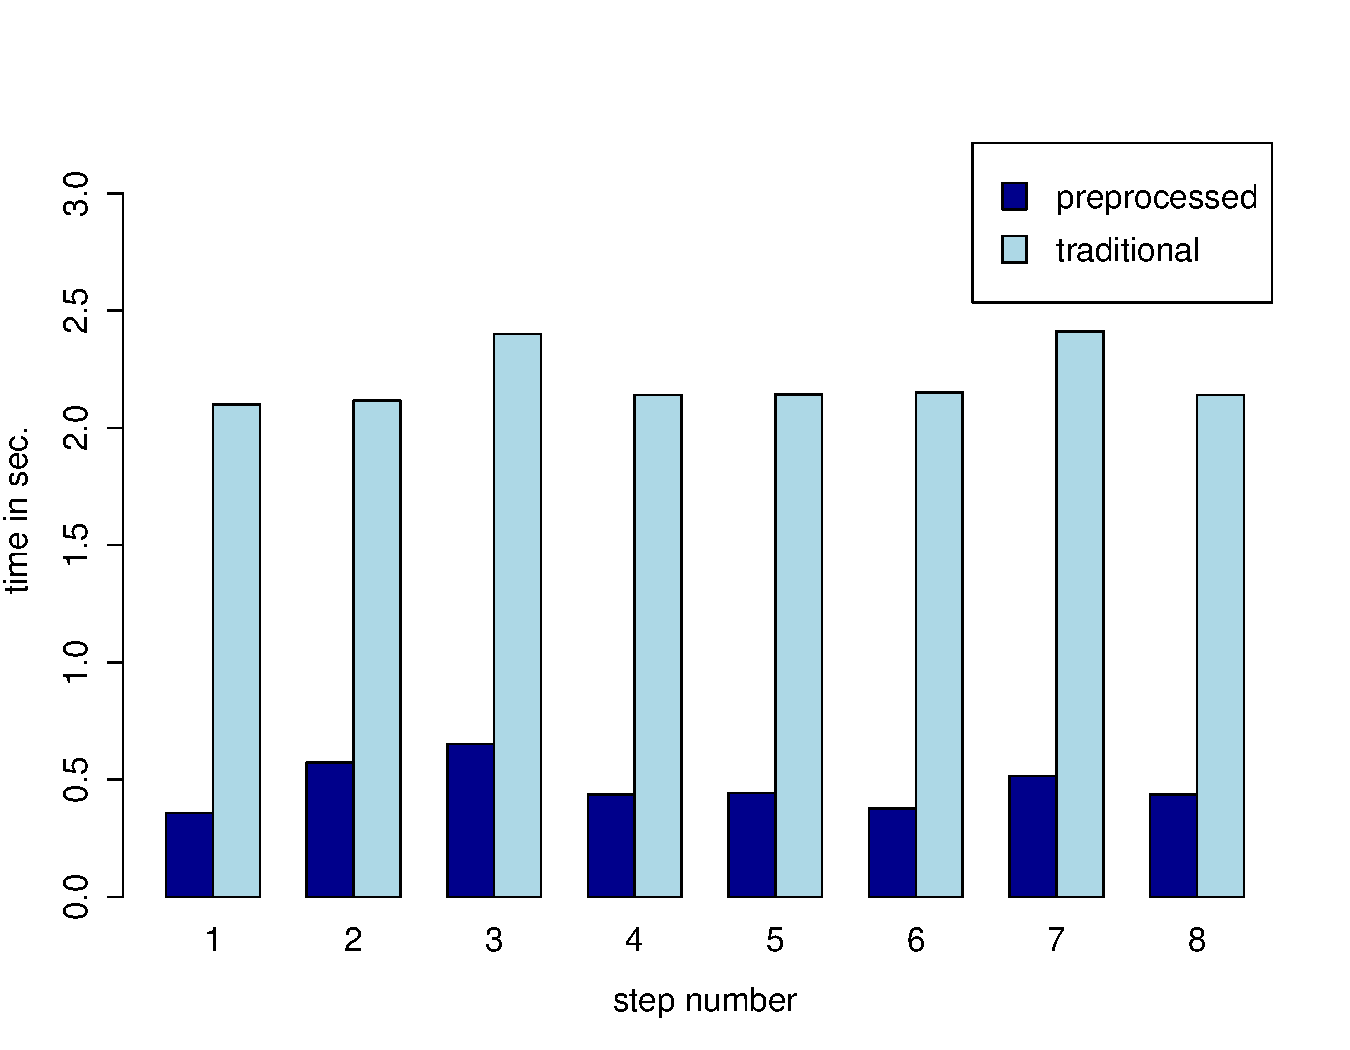
\includegraphics[width=0.5\textwidth]{Rplot26}
%     }
%   %  
%    % 
% %
% %
%     %}%\hfill
%     \subfloat[10 wards, reasoning time per event.\label{fig:results10ward}]{%
%       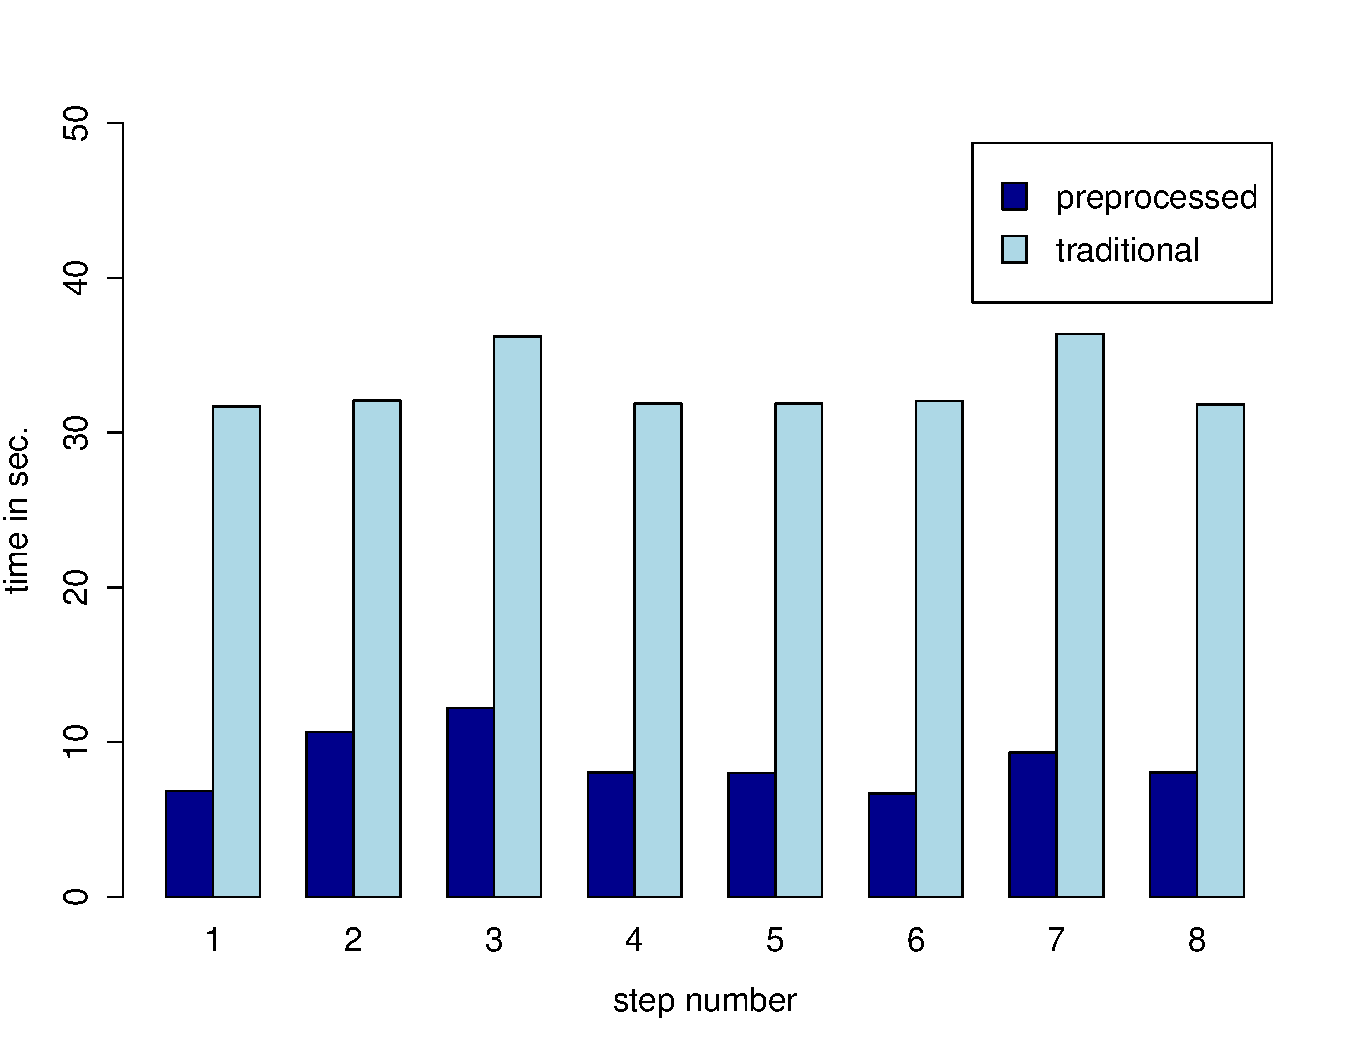
\includegraphics[width=0.5\textwidth]{Rplot27}
%     }
%     \caption{Comparison of reasoning times using preprocessed and traditional rules. The preprocessing step improves reasoning times.
%       }
%     \label{figure:results}
%   \end{figure}
%   
  
\begin{figure}
\centering
\begin{subfigure}{.5\textwidth}
  \centering
  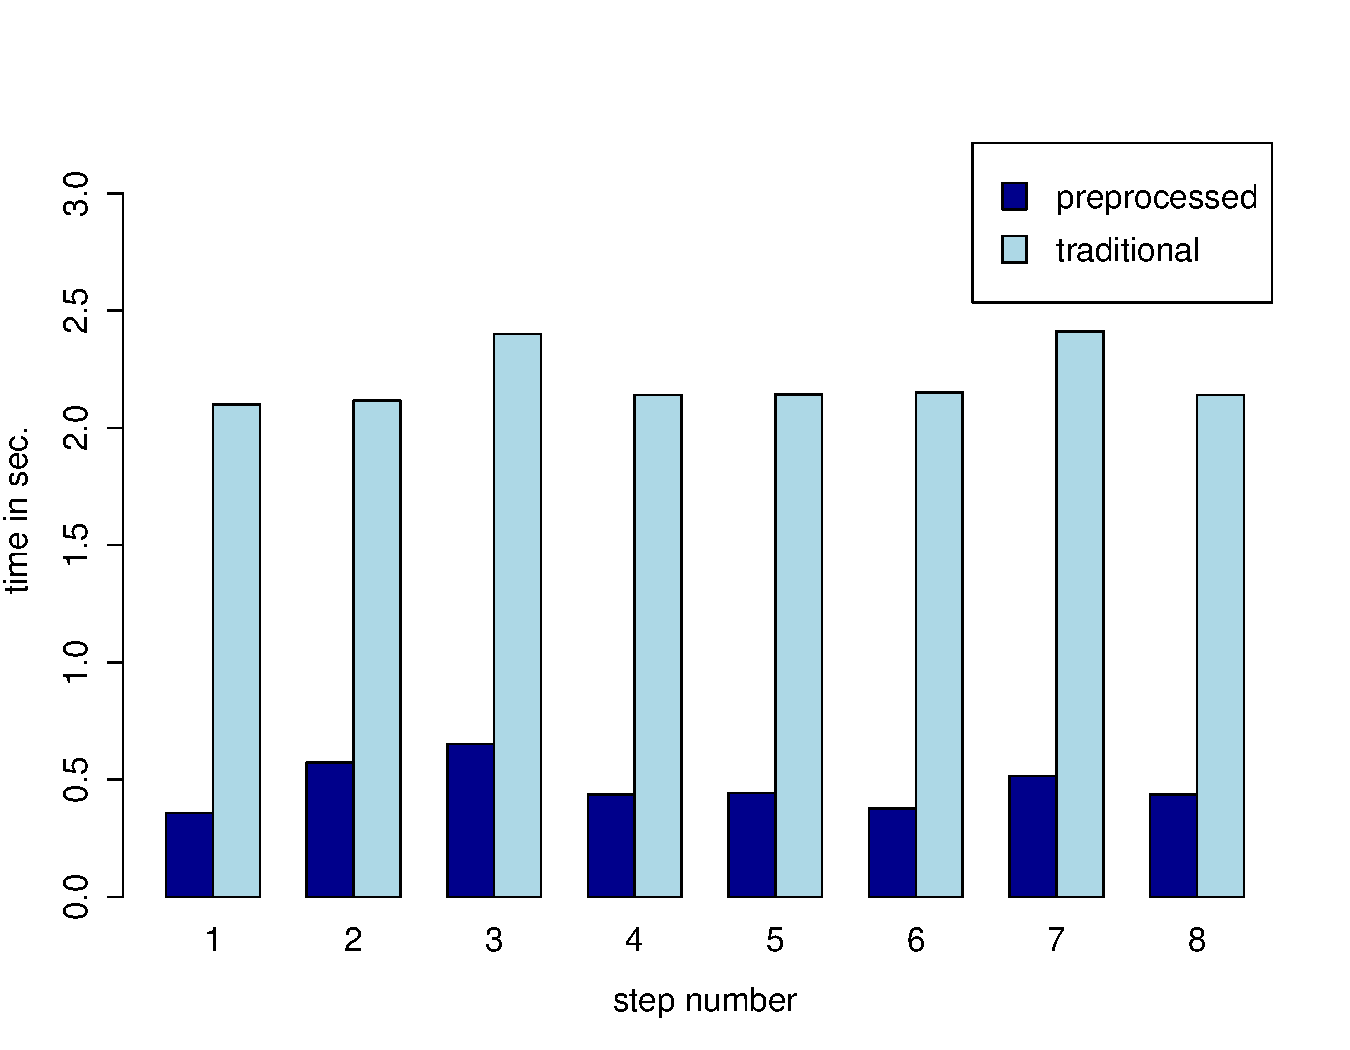
\includegraphics[width=\linewidth]{Rplot26}
  \caption{1 ward, reasoning time per event.}
  \label{fig:results1ward}
\end{subfigure}%
\begin{subfigure}{.5\textwidth}
  \centering
  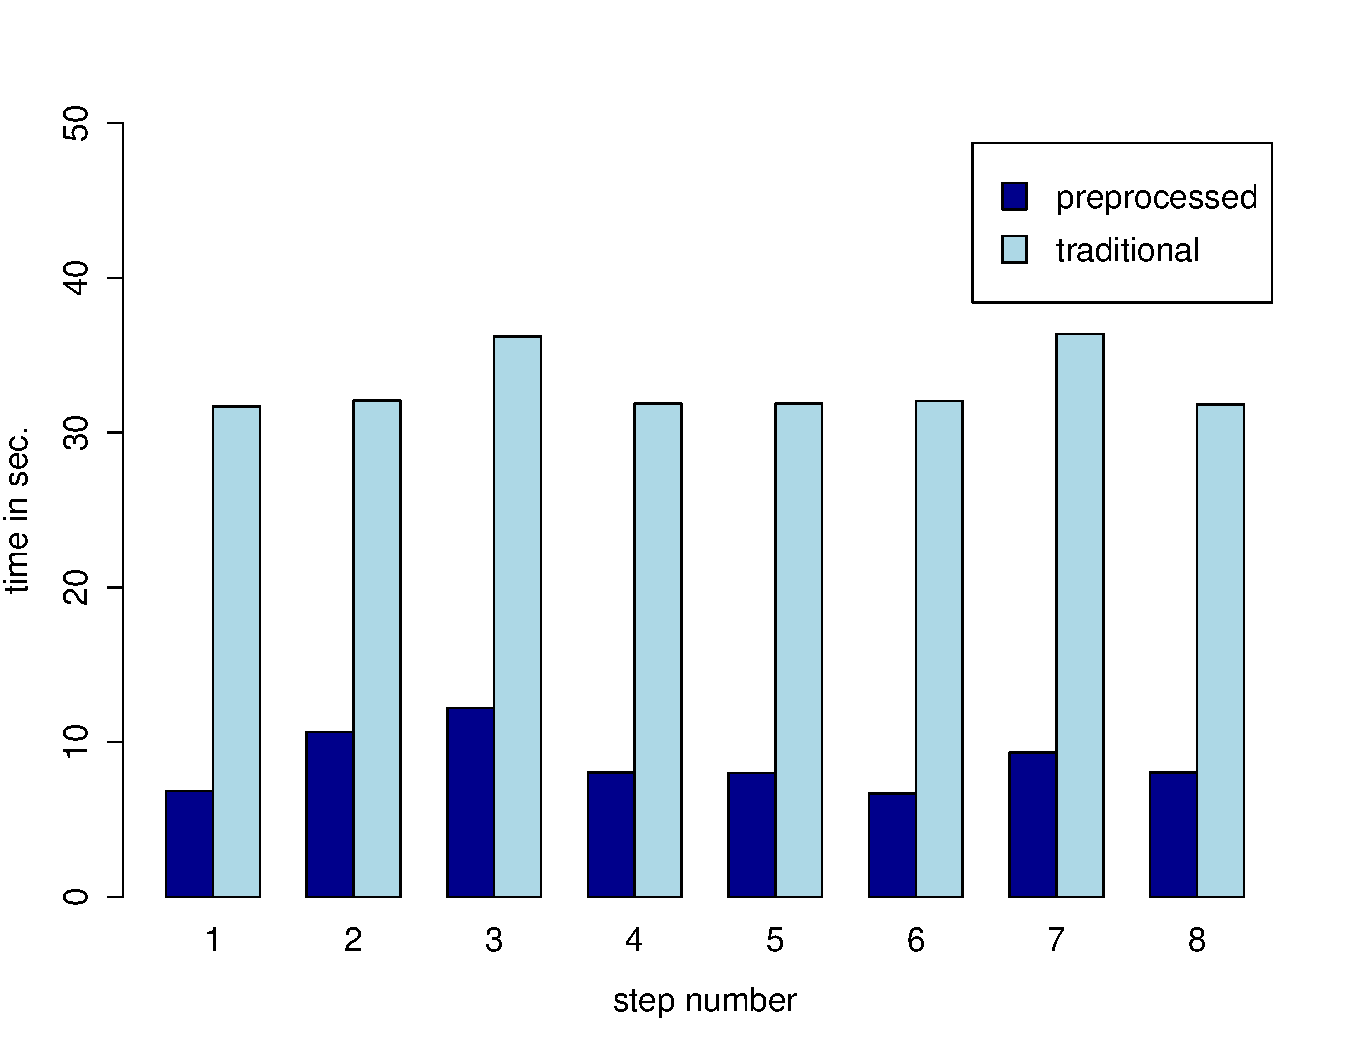
\includegraphics[width=\linewidth]{Rplot27}
  \caption{10 wards, reasoning time per event.}
  \label{fig:results10ward}
\end{subfigure}
\caption{Comparison of reasoning times using preprocessed and traditional rules. The preprocessing step improves reasoning times.}
\label{figure:results}
\end{figure} 
 

The figures show how preprocessing the rules improves reasoning times significantly,  consistently requiring only a quarter of the reasoning time.
This trend manifests itself regardless of the amount of dynamic data involved.
Whereas the traditional rule set can no longer be used in a hospital with 10 wards the 
preprocessed rule set still provides reasonable reasoning times. 
  

\subsection{Conclusion and Future Work}\label{conc}
In this paper we have shown that precomputing and using specialized rules based on the ontology's TBox improve reasoning times of OWL RL reasoning by about 75\%. 
The main cause
for that is that 
the newly computed rules are less complex---in terms of the variables which have to be unified during reasoning---than the
original version of the rules taken from the OWL RL 
profile description. 
Another aspect which makes reasoning faster in our set up is the fact that rules for concepts which are not even present in the ontology's TBox will not get 
produced by the preprocessing step. If for example the rather expensive concept \texttt{owl:sameAs} does not occur in any triple of the considered ontology,
no specialized rules will be produced for this concept.


The presented preprocessing step consists of two simple reasoning runs which can be performed before dealing with additional input data. Using the 
EYE reasoner this preprocessing normally takes only a few seconds. In set ups where the TBox does not change during run time the produced rules can be 
used whenever the ABox data to reason on changes as in the example introduced in this paper. Our approach is independent of the  reasoning done on top of the 
TBox by additional rules. This makes the rule version of the ontology's TBox even more suitable for reuse.


Our approach makes use of the special properties of Notation3 Logic.
By providing the option of using rules to produce new rules this logic is particularly suitable for our purposes. Furthermore Notation3 offers
multiple predicates to act on lists as for example the function \texttt{list:in}.
This eases the implementation of rule producing rules based on OWL predicates as there are many OWL constructs which are normally stated with lists 
in their object position.


Notation3 Logic posses other interesting properties which we are planning to apply in future work: in \nthree, rules can have existential variables in their 
consequence.
Using this particular property it will be possible to also cover OWL EL concepts which are not present in OWL RL. Similarly as done in 
for example OWLim \cite{elowlim} we are planning to include OWL EL in our implementation.  We furthermore want to investigate the actual costs of
processing the different OWL concepts by our newly produced rules. This will enable us to recommend the exclusion of particular concepts if not really needed. 


% $\forall x \exists $
% 
% \paragraph{\textbf{Acknowledgements}} The research activities described in this paper were funded by Ghent University, iMinds, the IWT Flanders, the FWO-Flanders, 
% and the European Union, in the context of the project ``ORCA'', which is a collaboration of Televic Healthcare, Internet-Based Communication Networks and Services (IBCN), and Multimedia Lab (MMLab).


% \FloatBarrier
% 
% 
% 
% \bibliographystyle{splncs03} 
% \bibliography{References} 
% 
% 
% 
% \end{document}

